
\section{Notationen}

Für eine Menge $\Omega$ bezeichnet $\# \Omega$ die Anzahl ihrer Elemente und $\mathcal{P} (\Omega) : = \{ A \, | \, A \subseteq \Omega \}$ die Potenzmenge von $\Omega$. 


\begin{figure}[htp]
      \centering
    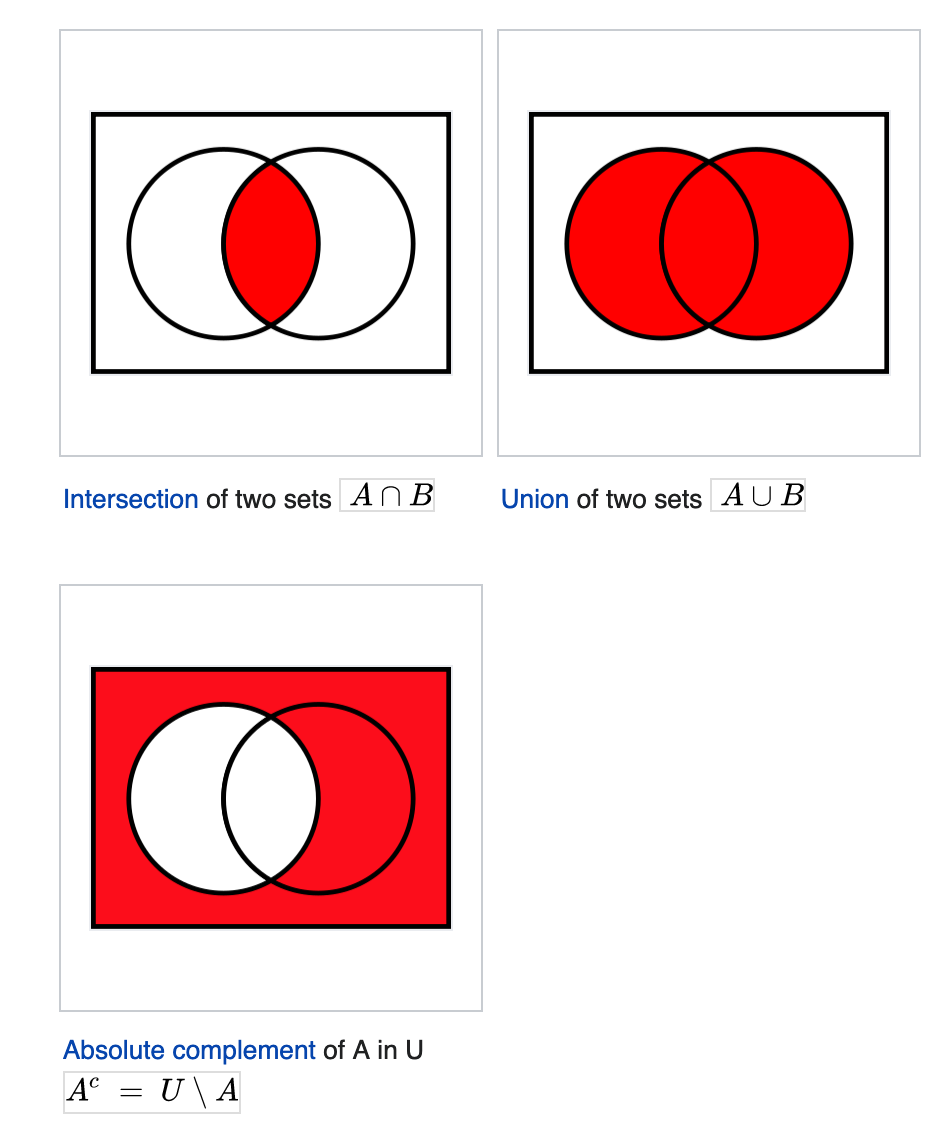
\includegraphics[width=0.9\textwidth]{images/Venn}

      \caption{Quelle: Wikipedia}
\end{figure}


\begin{figure}[htp]
      \centering
    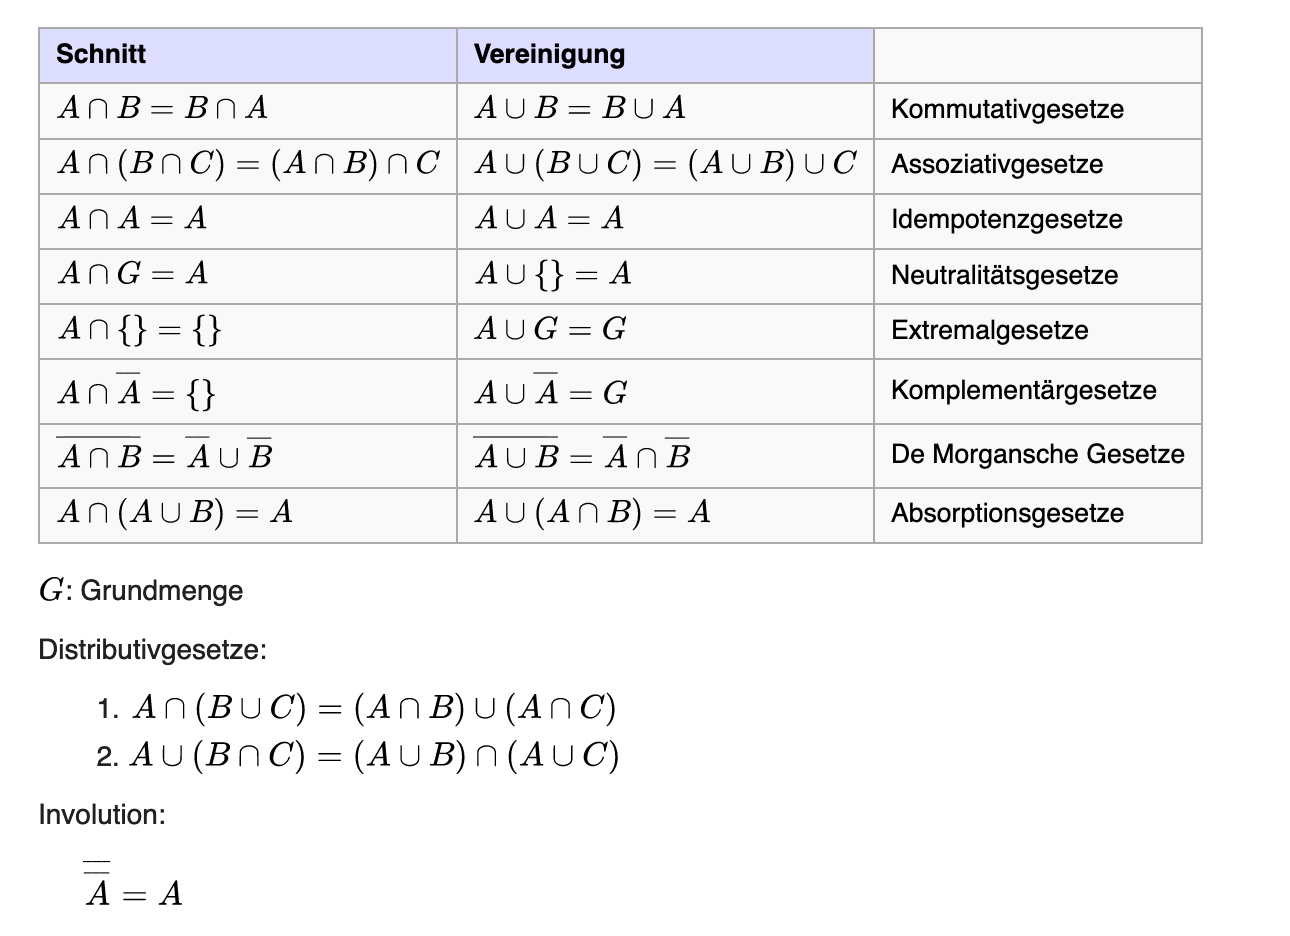
\includegraphics[width=0.9\textwidth]{images/mengengesetze}

      \caption{Quelle: Wikipedia}
\end{figure}



\newpage